% vim: spelllang=es

\chapter{Diseño}\label{sec:design}

\section{Arquitectura}

Para el sistema de plugins final, la estructura de Tremor debería ser la
descrita por la Figura~\ref{fig:separation}.

\begin{figure}
    \centering
    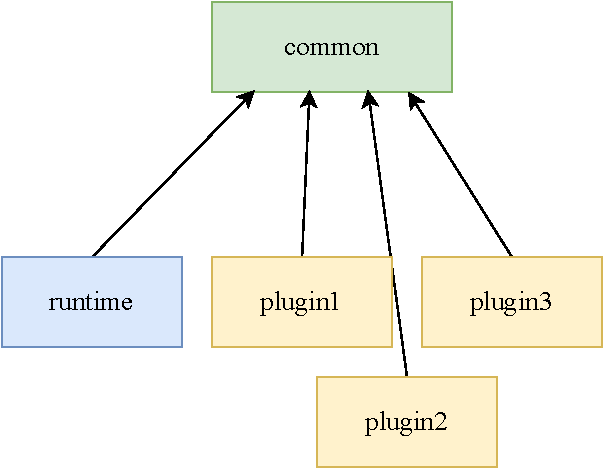
\includegraphics[width=7cm]{./Imagenes/separation.pdf}
    \caption{La estructura ideal para un sistema de plugins.}%
    \label{fig:separation}
\end{figure}

\begin{itemize}
    \item El binario \code{runtime}, que carga los plugins.

    \item Los binarios \code{plugin}, con las implementaciones de los
        componentes del sistema.

    \item La librería \code{common}, con la interfaz compartida entre la runtime
        y los plugins. Por tanto, ambos tipos de binario dependen de
        \code{common}.

\end{itemize}

Esta estructura es esencial para el objetivo principal: mejorar los tiempos de
compilación. Existen dos maneras de entender los tiempos de compilación: para el
desarrollo de la runtime y para el desarrollo de los plugins.

En ambos casos, se quiere compilar únicamente \emph{uno} de los componentes.
Para el desarrollo de un plugin, no debería hacer falta recompilar también la
runtime, porque no está siendo modificada. Y si se está trabajando sobre la
runtime, no debería recompilarse la funcionalidad de los plugins.

El problema reside en que, inicialmente, solo existe un binario con todo:
\code{runtime}, \code{plugin}s, y \code{common}. El primer paso debería ser el
que muestra la Figura~\ref{fig:separation_temporary}: separar los plugins del
mono-binario. La funcionalidad se encuentra en binarios diferentes, así que la
runtime tendrá un tiempo de compilación significativamente menor. Desarrollar un
plugin también será menos costoso, ya que no hará falta compilar los demás.

\begin{figure}
    \centering
    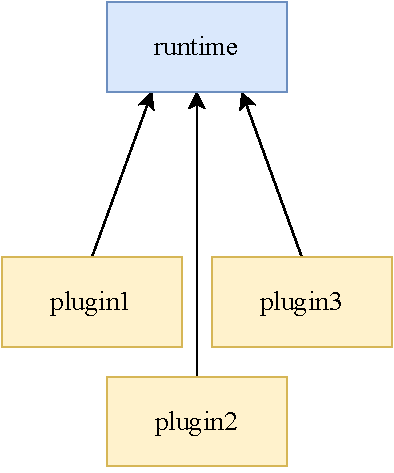
\includegraphics[width=6cm]{./Imagenes/separation-temporary.pdf}
    \caption{La estructura inicial del sistema de plugins para un desarrollo más
    rápido.}%
    \label{fig:separation_temporary}
\end{figure}

Para un tiempo de compilación óptimo también es necesario un segundo paso. La
interfaz del PDK sigue encontrándose junto a la runtime, así que un plugin
tendrá que compilar también la runtime, aun cuando no es necesario. Esto no será
una mejora tan grande sobre los tiempos de compilación como en el paso anterior,
dado que compilar la runtime es mucho menos costoso que compilar todos los
plugins.

Este segundo paso se puede omitir durante el inicio del proyecto, ya que la
interfaz está muy fuertemente relacionada con la runtime. Los tipos usados en la
interfaz tendrán que moverse a una librería distinta, pero al provenir todos de
la runtime, se tendrá que modularizar una gran parte del código. Cuantos menos
cambios se produzcan al principio del proyecto, mejor. Habrán menos conflictos y
resultará más fácil y seguro revisar el ćodigo en pequeñas en iteraciones, en
vez de una única revisión grande.

\section{Plan de desarrollo}

A partir de la sección anterior, se puede elaborar un plan aproximado para el
sistema de plugins basado en iteraciones (o pull requests):

\begin{enumerate}
    \item \textbf{Definir una nueva interfaz y usarla internamente}: el sistema
        de plugins debería ser lo más minimalista posible. La interfaz principal
        puede convertirse de forma que soporte plugins, pero se debería mantener
        todo en un mismo binario por simplicidad. La parte de cargado de plugins
        se puede dejar como una prueba de concepto por el momento y se pueden
        incluir algunos plugins externos para demostrar su funcionamiento.

        Esta iteración se podrá fusionar con la rama principal, ya que el
        programa seguirá funcionando de la misma forma, simplemente con una
        interfaz distinta para los conectores internamente.

    \item \textbf{Hacer los plugins externos}: dado que los plugins
        desarrollados usan la nueva interfaz, este paso debería ser sencillo.
        Requerirá reorganizar el repositorio con los binarios nuevos, arreglar
        el sistema de compilación y la integración continua, entre otros.

    \item \textbf{Separar la runtime de la interfaz}: como se ha explicado, esta
        parte es menos importante pero puede causar un gran número de cambios.
        Por tanto, solamente al final se separará la interfaz a una librería
        \code{common} nueva, para una última reducción de los tiempos de
        compilación.

    \item \textbf{Otras mejoras para el despliegue}: últimos cambios antes de
        incluir el sistema de plugins en la nueva versión, incluyendo una
        limpieza, optimizaciones, documentación o evaluar los resultados
        finales.

\end{enumerate}

\section{Tecnologías a considerar}

Esta sección describe las tecnologías más viables que se han considerado como
base para el PDK. Algunas no cumplirán los requisitos mencionados anteriormente,
pero es necesario asegurarse antes de escribir ninguna línea de código.

\subsection{Lenguajes interpretados}

Es frecuente el uso de lenguajes interpretados para extender la funcionalidad de
un programa a tiempo de ejecución: Python, Perl, JavaScript, etc.
Particularmente, el editor de texto \namecite{vim} creó su propio lenguaje,
VimScript, para poderlo personalizar por completo. Ahora \namecite{neovim}, un
fork más moderno, está esforzándose por tener Lua como lenguaje de primera clase
para su configuración~\cite{nvimlua}. Incluso Tremor tiene su propio lenguaje
para el procesado de eventos e inicialización.

De todos los lenguajes disponibles, Lua sería una de las mejores opciones para
este sistema de plugins en específico. Está hecho con \emph{embedding} en mente:
es muy sencillo y únicamente ocupa alrededor de
220KB~\cite{ierusalimschy2006programming}. Algunas implementaciones del
lenguaje, como LuaJIT, son extremadamente eficientes y pueden ser viables hasta
en escenarios de rendimiento crítico~\cite{luajitperf}. Adicionalmente, las
garantías de seguridad de Lua son más fuertes que otros lenguajes, dado que no
requiere \unsafe e incluye una \sandbox (aunque es ``delicada y difícil de
configurar correctamente'')~\cite{luasandboxes}.

Rust dispone de librerías como \namecite{rlua}, que parece enfocar su interfaz
en ser idiomática y segura, que es un punto positivo para un lenguaje que usa C
internamente. Desgraciadamente, parece estar semi-abandonada y fue reemplazada
por \namecite{mlua}. Por lo general, el ecosistema de Lua en Rust no parece lo
suficientemente maduro para un proyecto como este y aún queda trabajo para
mejorar su estabilidad.

También sería posible usar uno de los lenguajes interpretados creados
específicamente para Rust: \namecite{gluon}, \namecite{rhai} o \namecite{rune}.
Usarlos posiblemente resulte en código más limpio y simple. Sin embargo, el
ecosistema todavía está en su infancia y ninguna de las opciones son tan
estables ni seguras como lenguajes de programación de propósito general. Rhai,
el más usado, anunció su versión v1.0 en julio de 2021 y no sobrepasa las
200.000 descargas, mientras que Lua fue creado en 1993 y es uno de los 20
lenguajes más famosos, según el \namecite{tiobe}.

De cualquier manera, portar el código a este sistema de plugins sería un trabajo
excesivamente laborioso. Todos los conectores tendrían que reescribirse por
completo a un lenguaje distinto. Para un proyecto nuevo sería una alternativa
interesante, pero ciertamente no lo es en el caso de Tremor.

\subsection{WebAssembly}

\namecite{wasm}, también conocido como Wasm, es esencialmente un formato binario
abierto y portable. A diferencia de binarios normales, el mismo ejecutable Wasm
puede correr en cualquier plataforma, siempre y cuando exista una runtime que lo
soporte. Comenzó como una alternativa a JavaScript exclusiva a la web, pero ha
evolucionado con el tiempo y ahora es posible usarlo en el escritorio gracias a
la interfaz \namecite{wasi}.

El objetivo de Wasm es maximizar la portabilidad y seguridad, sin un coste de
rendimiento excesivo. Su diseño incluye una \sandbox para lidiar con programas
no fiables, como suele ocurrir con plugins, y apenas no requiere usar \unsafe.
Aunque técnicamente sea interpretado también, el código existente en Tremor sí
que podría ser reusado, ya que es compilado desde otros lenguajes como Rust o C.

Existen dos runtimes principales para Rust: \namecite{wasmer} y
\namecite{wasmtime}. Ambas son implementaciones competitivas enfocadas a unos u
otros casos de uso. Por lo general, Wasmer es más adecuado para embebirlo en
programas nativos y Wasmtime se centra en los programas independientes, aunque
los dos se pueden usar apara ambos casos~\cite{wasmwikiusage}.

WebAssembly todavía es una tecnología relativamente nueva, así que algunas
partes siguen bajo desarrollo continuo y necesitan mejoras, como en rendimiento.
En comparación a JavaScript, \textcite{jangda2019not} muestra resultados
mezclados al realizar pruebas de rendimiento. Depende principalmente de de la
runtime y del entorno que se esté usando, variando desde mejoras en velocidad de
1.67x en Chrome, a 11.71x con Firefox. Cuando se compara con código nativo,
\textcite{libsodiumwasmperf} describe una varianza similar, donde Wasmer es
2.47x más lento y con Wasmtime es 3.28x. Aunque WebAssembly es una solución más
eficiente que algunos lenguajes interpretados, sigue sin llegar al nivel de
binarios nativos, y quizá no sea suficiente para este proyecto.

Esta tecnología es de las más adecuadas en esta sección; su único punto flojo es
el rendimiento. Tras implementar algún sistema de plugins en miniatura, su
usabilidad y seguridad era excelente. Si fuera posible transferir datos (tipos
no triviales) entre la runtime y el plugin sin tener que copiarlos ni
serializarlos, definitivamente merecería la pena usarlo. La especificación de
WebAssembly define únicamente enteros y decimales como sus tipos
disponibles~\cite{wasmertypes}. Existen algunas maneras de tratar tipos
compuestos, como estructuras o enumeraciones:

\begin{itemize}
    \item A través de la \namecite{wasminterfacetypes}. Esta define un formato
        binario para codificar y decodificar tipos nuevos: números más
        especializados, caracteres individuales, listas, estructuras y
        enumeraciones. También especifica una serie de instrucciones para
        transformar los datos entre WebAssembly y el mundo exterior.

        Notar que esta propuesta no intenta definir una representación fija de,
        por ejemplo, una cadena de caracteres en Wasm; intenta permitir tipos de
        alto nivel agnósticos a su representación. Las interfaces se pueden
        definir independientemente del lenguaje de programación que se esté
        usando, gracias al formato \namecite{witx}, como muestra la
        Figura~\ref{fig:witx_example}.

        El mayor problema de esta solución es que aún está en ``Fase 1'': aún
        necesita mucho trabajo y su especificación no es estable. Ninguna de las
        runtimes tienen soporte para esta propuesta
        aún~\cite{interfacetypeswasmtime}\cite{interfacetypeswasmer}. Tras
        fallar al intentar usarlo, esta opción fue descartada.

    \item El método más popular actualmente, que es funcional pero imperfecto,
        con punteros y memoria compartida. El usuario debe construir y
        serializar el tipo compuesto y después guardarlo en la memoria reservada
        para Wasm, a la que la runtime puede acceder directamente con punteros.
        Esto es lo que otros sistemas de plugins como Feather o Veloren
        hacen~\cite{featherpluginsystem}\cite{velorenpluginsystem}, así que es
        garantizado que funciona.

        No sólo requiere un paso de serialización y otro de deserialización y
        escribir y leer todos los datos de una memoria, sino que también es una
        tarea ardua y complicada de hacer correctamente. No es algo que Tremor
        se pueda permitir por tener un rendimiento pobre.

    \item Otra opción que emplean programas como
        Zellij~\cite{zellijpluginsystem}, que usa un ejecutable de Wasm en vez
        de usarlo como una librería importable. Para cargarlo, ejecuta el
        binario independiente y usa \stdin y \stdout para los flujos de datos.
        Desgraciadamente, esto también requiere serializar y copiar datos, y
        tiene que descartarse.

\end{itemize}

\begin{figure}
    \centering
    \begin{minted}{lisp}
(use "errno.witx")

;;; Add two integers
(module $calculator
  (@interface func (export "add")
    (param $lh s32)
    (param $rh s32)
    (result $error $errno)
    (result $res s32)
  )
)
    \end{minted}
    \caption{Ejemplo de interfaz definida con \code{witx}.}%
    \label{fig:witx_example}
\end{figure}

\subsection{eBPF}

eBPF es ``una tecnología revolucionaria con orígenes en el kernel de Linux que
puede ejecutar programas en \sandbox en el kernel de un sistema
operativo''~\cite{ebpf}. Posee muchas similitudes a WebAssembly: funciona
definiendo una serie de instrucciones que pueden ejecutarse por una máquina
virtual y ha evolucionado para que sea posible usarlo fuera del kernel, en
espacio de usuario.

Esta tecnología es prometedora, ya que a diferencia de WebAssembly, no es
necesario serializar los datos o escribirlos a una memoria intermedia. Ya que
existe control completo sobre la máquina virtual, la runtime podría implementar
una \sandbox personalizada para comprobar las direcciones de memoria de donde se
lee o escribe, asegurándose de que se encuentran en el rango permitiendo y
pudiendo compartir una única memoria. La penalización en el rendimiento sería
interpretar las instrucciones en vez de ejecutar código nativo, pero
técnicamente Tremor sí que podría usarlo.

El problema principal con eBPF es la carencia de soporte en Rust. La mayoría de
sus usuarios usan C y lo muestra la poca cantidad de tutoriales, guías,
artículos o incluso librerías disponibles para Rust. No es posible compilar Rust
a instrucciones eBPF de forma oficial y la única runtime disponible es
\namecite{rbpf} y derivados como \namecite{solana_rbpf}, ya que este primero
parece estar obsoleto. Además, supondría un esfuerzo mucho mayor que
WebAssembly, ya que también requeriría implementar una \sandbox personalizada.

\subsection{Cargado dinámico}\label{sec:dynload}

El cargado dinámico es el método más popular para implementar un sistema de
plugins, especialmente para el lenguaje de programación C. Consiste en acceder
directamente a recursos en objetos compilados por separado, aun después de la
fase de \emph{linking}. Es una de las opciones más eficientes porque no impone
casi ningún coste adicional tras el cargado del plugin en la memoria de la
runtime, y no requiere crear procesos o hilos nuevos.

La librería principal en Rust es \namecite{libloading}, aunque también existen
las menos conocidas \namecite{dlopen} y \namecite{sharedlib} con pequeñas
diferencias entre sí~\cite{cratesdynloadcompare}. Por desgracia, todas emplean
\unsafe extensivamente tanto en su implementación como en su interfaz, son
complicadas de usar correctamente~\cite{hardplugins1}\cite{hardplugins2},
incluyen sutiles disparidades entre sistemas operativos~\cite{hardplugins3}, y
no disponen de un mecanismo para aislar a los plugins. La única manera de
mejorar la usabilidad será a través de los macros, herramientas y abstracciones
facilitados por ellas mismas y otras librerías.

\subsubsection{Estabilidad del ABI}\label{sec:abi}

El problema más importante de esta alternativa es que Rust carece de una
\emph{Interfaz Binaria de Aplicación~(ABI)} estable. El ABI es una interfaz
entre dos módulos binarios, en nuestro caso entre un ejecutable (runtime) y una
librería dinámica (plugin). Se encarga de especificar, entre otros, la
estructura que siguen los tipos en memoria y la convención usada para llamar
funciones. Sin un ABI concreto definido (y por tanto, sin \emph{estabilidad}),
es imposible saber cómo acceder a los recursos de los plugins. Esto sucede con
cualquier tecnología que interactúe con datos de otros binarios directamente,
como eBPF o memoria compartida.

Al comenzar este proyecto, gran cantidad de fuentes en la comunidad confundían
qué significa la inestabilidad del ABI en
Rust~\cite{wrongabi1}\cite{wrongabi2}\cite{wrongabi3}\cite{dynloading1}. Este
popular malentendido también se dio en la propuesta del PDK y no nos dimos
cuenta del verdadero significado hasta haber invertido numerosas horas. El
equipo de Tremor --- yo incluido --- creía que el ABI de Rust es estable,
siempre que los dos binarios se compilen con exactamente la misma versión de
compilador. Esto resultó ser incorrecto, y fuentes como la referencia oficial no
entran en suficiente detalle sobre el tema~\cite[Application Binary Interface
(ABI)]{rustref}. Debe recurrirse a otra sección en la referencia, que menciona
brevemente lo siguiente:

``La estructura de tipos en memoria puede cambiar con cada compilación. En vez
de intentar documentar exactamente qué se hace, se documenta solo lo que se
garantiza hoy''~\cite[Type Layout]{rustref}

Esta asunción incorrecta se basa en que, hasta el momento, Rust no ha
implementado ninguna optimización que rompa el ABI entre ejecuciones de un
compilador de la misma versión. Pero no existe absolutamente ninguna garantía de
que esto sea así, y es un detalle de implementación del compilador del que no
debería confiarse. Es posible que este comportamiento sí que se rompa en el
futuro~\cite{randomizelayout}, en cuyo caso el sistema de plugins dejaría de
funcionar por completo.

Descubrir esto implicó un cambio de planes y un aumento muy notable en la
complejidad del proyecto. Ahora tendría que recurrirse a una ABI que sí que
tuviera garantías de estabilidad, y traducir entre la de Rust y esta para
comunicarse entre runtime y plugins. El ABI más conocido es el del lenguaje de
programación C, que tiene soporte integrado en Rust, como muestran las
Figuras~\ref{fig:rustpure}~y~\ref{fig:rustffi}.

\begin{figure}
    \centering
    \begin{minted}{rust}
pub struct Event {
    pub count: i32,
    pub name: &'static str,
}

pub fn transform(x: Event) -> i32 {
    println!("Se ha recibido el evento {}", x.count);
    x.count
}

pub static cached: Event = Event {
    count: 0,
    name: "mis datos"
};
    \end{minted}

    \caption{Ejemplo de cómo sería un plugin escrito con Rust.}%
    \label{fig:rustpure}
\end{figure}

\begin{figure}
    \centering
    \begin{minted}{rust}
#[repr(C)]
pub struct Event {
    pub count: i32,
    pub name: *const std::os::raw::char_c,
}

pub extern "C" fn transform(x: Event) -> i32 {
    println!("Se ha recibido el evento {}", x.count);
    x.count
}

#[no_mangle]
pub static cached: Event = Event {
    count: 0,
    name: "mis datos".as_ptr() as _
};
    \end{minted}

    \caption{El mismo plugin que la Figura~\ref{fig:rustpure}, pero usando el
    ABI de C.}%
    \label{fig:rustffi}
\end{figure}

\subsubsection{Razonamiento sobre la inestabilidad}

El hecho de que Rust no tenga un ABI bien definido es una decisión un tanto
controversial. En comparación, el estándar de C++ no especifica un ABI concreto,
pero sus compiladores intentan mantenerlo retrocompatible. Por tanto, aunque
rompería al probarse con compiladores distintos y en algunos casos
especiales~\cite{cpp_abi_problems}, técnicamente sí que es posible implementar
un sistema de plugins sin tener que pasar por C.

Sin embargo, esta retrocompatibilidad también causa problemas en el diseño de
C++ y obstaculiza su evolución~\cite{cpp_dead_std}. El tener un ABI estable
imposibilita la actualización interna de su librería estándar, resultando en
implementaciones obsoletas sin arreglo. Las expresiones regulares en C++ son
famosamente lentas, incluso peor que en lenguajes como
Python~\cite{cpp_vs_python_regex1}\cite{cpp_vs_python_regex2} o
Java~\cite{cpp_vs_java_regex}, pero no se podrán mejorar hasta que C++ decida
romper el ABI.

Rust intenta aprender de la situación de C++ y explícitamente no define ningún
ABI. Esto dificulta considerablemente llevar a cabo este proyecto y otros
similares, pero dinamiza la inclusión de nuevos arreglos u optimizaciones en sus
estructuras de datos. Por ejemplo, el mútex de la librería estándar era
subóptimo y había que recurrir a dependencias como \namecite{parking_lot} para
alcanzar un rendimiento máximo. Gracias a la inestabilidad del ABI, se pudo
modificar el código interno transparentemente e incluir las mejoras en una nueva
versión. Esto se ha repetido múltiples veces, también reemplazando por completo
la implementación de \rust{HashMap} con un nuevo método más eficiente inventado
en Google~\cite{rust_replace_map}\cite{hashbrown}.

\subsubsection{Herramientas disponibles}

La viabilidad del cargado dinámico se basa en una librería de más alto nivel,
\namecite{abi_stable}. Esta usa \code{libloading} internamente y exporta una
gran cantidad de macros y herramientas para facilitar el desarrollo. Incluye una
copia de la librería estándar de Rust declarada con el ABI de C, con nombres
generalmente precedidos por la letra \code{R}. Por tanto, en vez del vector
\rust{Vec<T>}, podremos usar \rust{RVec<T>}; en caso contrario habría que
recurrir a punteros (\rust{*const T}) o tendríamos que reescribir los tipos
desde cero nosotros. También da soporte para librerías externas muy conocidas en
la comunidad, como \namecite{crossbeam} o \namecite{serde_json}. La
Figura~\ref{fig:rustabi_stable} demuestra parte de la simplificación respecto al
código en la Figura~\ref{fig:rustffi}.

Existen más alternativas o extensiones para el cargado dinámico que se tuvieron
en cuenta, como \namecite{lccc}, \namecite{safer_ffi} o \namecite{cglue}, pero
no son soluciones tan completas ni maduras, por lo que no se usarán en este
proyecto. \abistable se trata de una librería grande, con más de 50.000 líneas
de código en Rust (como referencia, Tremor tiene unas 35.000 líneas), por lo que
el aumento de complejidad deberá tenerse en cuenta en la decisión de la
tecnología final a usar.

\begin{figure}
    \centering
    \begin{minted}{rust}
#[repr(C)]
#[derive(StableAbi)]
pub struct Event {
    pub count: i32,
    pub name: RStr<'static>,
}

#[sabi_extern_fn]
pub fn transform(x: Event) -> i32 {
    println!("Se ha recibido el evento {}", x.count);
    x.count
}
    \end{minted}

    \caption{El mismo plugin que la Figura~\ref{fig:rustpure}, pero con
        \abistable. La declaración de la global \rust{cached} se omite por
        simplicidad.}%
    \label{fig:rustabi_stable}
\end{figure}

\subsection{Comunicación Inter-Proceso}

Otra opción popular para sistemas de plugins es la \emph{Comunicación
Inter-Proceso}, que divide el programa en procesos distintos de tipo cliente y
servidor. El cliente actuaría como runtime y estaría conectado a múltiples
servidores que proporcionan la funcionalidad. Se podría comparar con el
\emph{Language Server Protocol}~\cite{lsp}, basado en JSON-RPC y usado por la
mayoría de editores de texto para tener soporte especializado para cualquier
lenguaje de programación.

Una ventaja común para todos los métodos de esta familia es que los plugins se
podrán escribir en Rust, así que el código existente se podría reusar. Además,
ya que el cliente y servidor se dividirían en múltiples procesos, serían más
seguros por lo general; plugins defectuosos no afectarían a la runtime de
Tremor.

\subsubsection{Sockets}

Son los que peor rendimiento tienen de acuerdo a la Figura
\ref{fig:ipc_comparison1} y la Figura \ref{fig:ipc_comparison2}, pero también
son los más famosos, y consecuentemente, los más probados y fáciles de usar. Los
\sockets son la misma tecnología usada en cualquier servidor para comunicarse
con un cliente y viceversa, por lo que hay una cantidad enorme de
implementaciones disponibles.

\begin{figure}
    \centering
    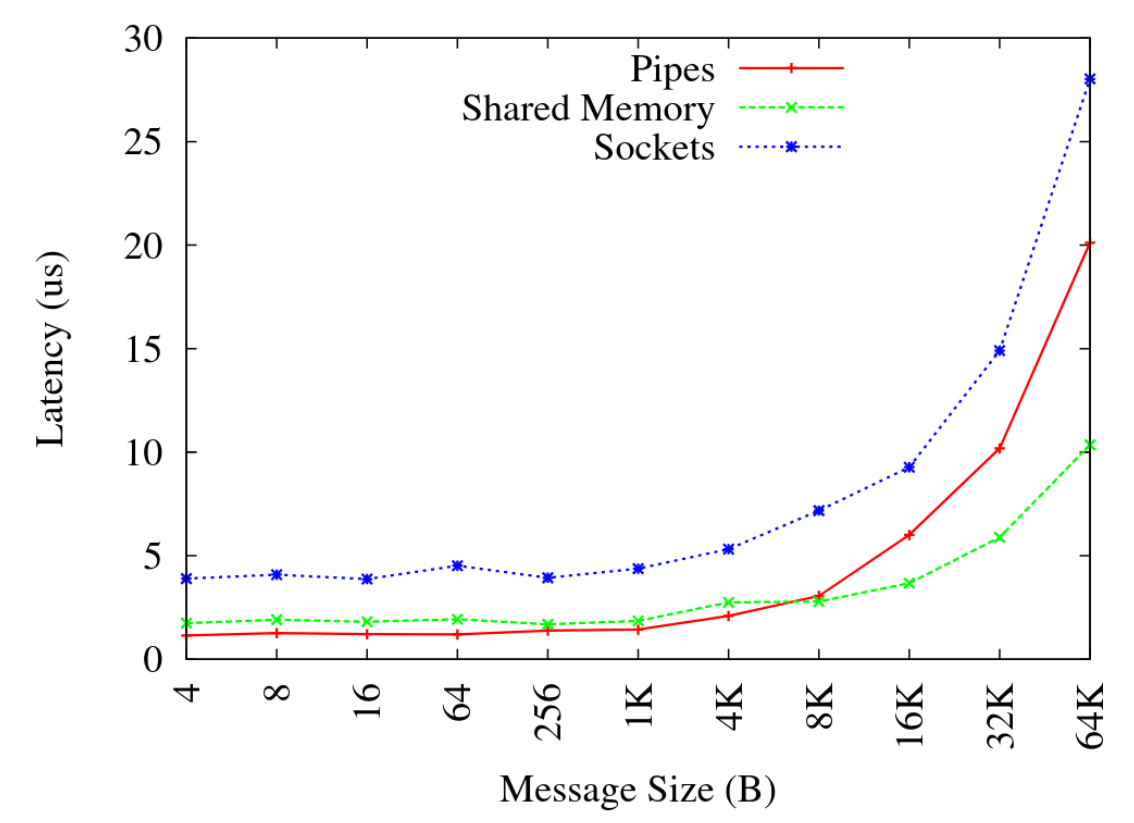
\includegraphics[width=12cm]{./Imagenes/venkataraman2015evaluation1.png}
    \caption{Latencia vs. Tamaño de Mensaje \cite{venkataraman2015evaluation}.}%
    \label{fig:ipc_comparison1}
\end{figure}

\begin{figure}
    \centering
    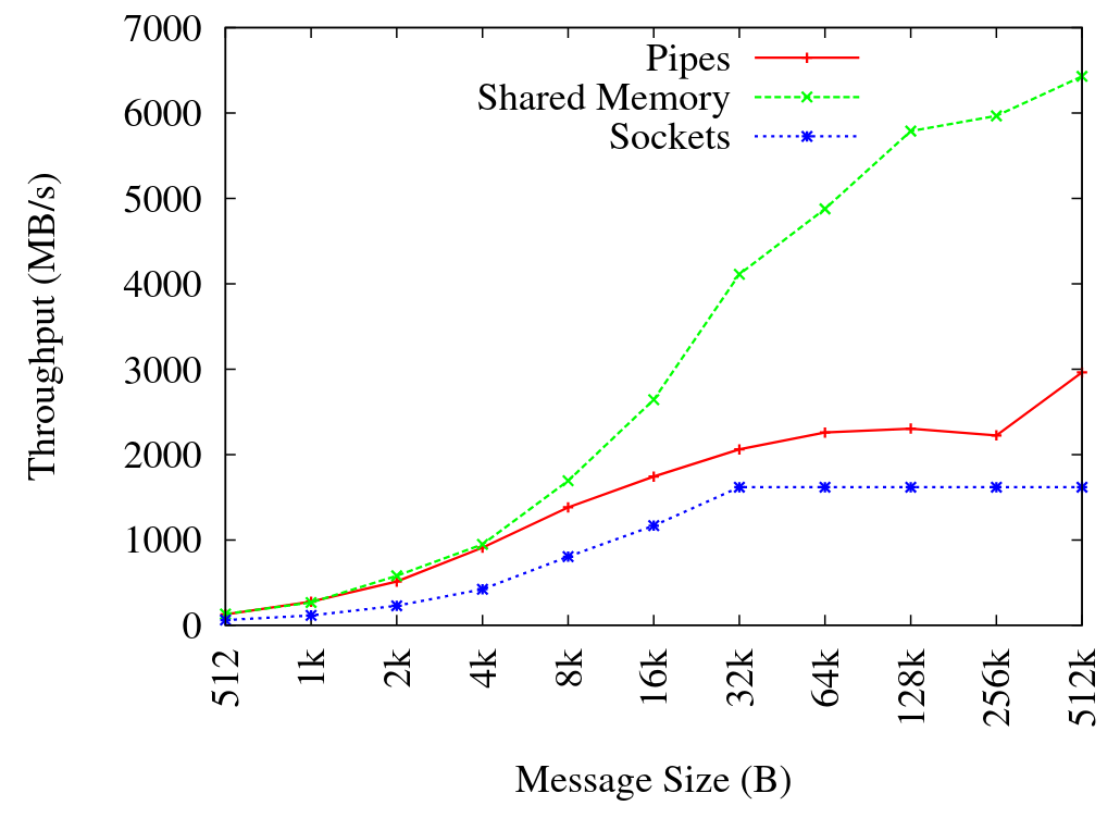
\includegraphics[width=12cm]{./Imagenes/venkataraman2015evaluation2.png}
    \caption{Rendimiento vs. Tamaño de Mensaje
    \cite{venkataraman2015evaluation}.}%
    \label{fig:ipc_comparison2}
\end{figure}

Usar \sockets también requiere un paso de serialización, dado que los datos se
envían en paquetes entre procesos. Formatos como JSON son los más flexibles,
pero otros como \namecite{protobuf} prioritizan la eficiencia.

\subsubsection{Pipes}

Para un sistema de plugins, las \pipes son muy similares a los \sockets, cuya
única diferencia es que las \pipes solo se pueden usar en una misma máquina. Con
\sockets, técnicamente podrías usar TCP o UDP y tener la runtime y los plugins
en ordenadores distintos. Esto no es algo necesario para el caso de Tremor, y ya
que las \pipes ofrecen un mejor rendimiento, posiblemente sean una mejor opción
por lo general.

Por ejemplo, el gestor de archivos \namecite{nnn} usa este método: los plugins
pueden leer de una FIFO (una \pipe con nombre) para recibir las selecciones de
archivos o directorios que realice el usuario e implementar una funcionalidad
personalizada.

La única desventaja es que no parecen haber librerías populares para la
funcionalidad genérica de \pipes (quizá \namecite{interprocess} o
\namecite{ipipe}). Sin embargo, esto podría ser innecesario si se usaran las
\pipes de \stdin, \stdout o \stderr implícitamente, ya que tienen soporte en la
librería estándar al ejecutar comandos \emph{shell}~\cite[Pipes]{rustexample}.

\subsubsection{Memoria compartida}

Como el nombre indica, la memoria compartida consiste en inicializar un buffer
del que se puede leer y escribir desde dos o más procesos al mismo tiempo para
comunicarse. El API de memoria compartida se implementa a nivel del kernel, por
lo que depende mucho del sistema operativo y quizá no sea tan portable como
otras soluciones.

Tal y como indican las
Figuras~\ref{fig:ipc_comparison1}~y~\ref{fig:ipc_comparison2}, es el método con
mejor rendimiento, ya que no requiere copiar ni transformar datos. Los únicos
costes adicionales son el tener múltiples procesos y la inicialización de las
páginas compartidas en el sistema operativo, que se debe hacer únicamente al
principio~\cite{sharedmemperf}.

Desgraciadamente, el soporte para memoria compartida en Rust es casi
inexistente. Las únicas librerías disponibles son \namecite{shared_memory} y
\namecite{raw_sync}, que no superan las 150.000 descargas en total y usan gran
cantidad de \unsafe. Esto probablemente tenga que ver con el hecho de que
comparte los mismos problemas que cargado dinámico respecto a estabilidad de ABI
(explicado en la sección~\ref{sec:dynload}). No parece ofrecer nada mejor que el
cargado dinámico y por tanto se descarta como opción.

\section{Sistemas de plugins de referencia}

Otro punto de estudio importante es qué plugins ya hay existentes en Rust y cómo
se han realizado:

\begin{itemize}
    \item \namecite{cargo} o \namecite{mdbook} implementan un sistema de
        extensiones a través de la línea de comandos. Añadir un subcomando nuevo
        es tan sencillo como crear un binario con un prefijo establecido (por
        ejemplo, \code{cargo-expand}). Si este binario está disponible en la
        variable de entorno \code{PATH} al ejecutar \code{cargo}, se podrá
        invocar al plugin con \code{cargo expand} también. Es una implementación
        especialmente simple con \pipes e IPC, dado que usa \stdin y \stdout
        para comunicarse con la runtime.

    \item \namecite{zellij} es un entorno de trabajo en el terminal con ``un
        sistema de plugins que permite crear plugins en cualquier lenguaje que
        compile a WebAssembly''. De forma similar al caso anterior, funciona un
        binario distinto para cada plugin y la runtime ejecuta el código en
        WebAssembly, comunicándose con \stdin y \stdout.

    \item \namecite{xi} es un editor de texto moderno ahora abandonado. Usaba
        RPC con mensajes JSON para comunicarse con plugins en procesos
        distintos~\cite{xiplugin}, método también usado en Visual Studio
        Code~\cite{vscodeplugin} o Eclipse~\cite{eclipseplugin}.

    \item \namecite{bevy} es un motor de videojuegos cuyas prestaciones se
        implementan como plugins. En la mayoría de los casos, se cargan en
        tiempo de compilación, pero \rust{bevy::dynamic_plugin} da la
        posibilidad de hacerlo dinámicamente. Bevy se basa en la falsa
        estabilidad del ABI, así que podría romperse en un futuro.

        Otras fuentes como \textcite{dynloading1} o \textcite{dynloading2}
        también intentan usar cargado dinámico para funcionalidades similares.
        Este último se trata de \namecite{amethyst}, el predecesor de Bevy, que
        acabó rindiéndose debido a la inestabilidad del
        ABI~\cite{dynloading_giveup1}\cite{dynloading_giveup2}.

\end{itemize}

\section{Elección Final}

Tras implementar varios sistemas de plugins en miniatura con las tecnologías más
prometedoras mencionadas en esta sección, se tomó la decisión de usar cargado
dinámico con \abistable. Cada alternativa tiene sus puntos fuertes y sus puntos
flojos, como ilustra la Figura~\ref{fig:triangle}, pero pocas realmente
cumplen los requisitos de rendimiento establecidos por el equipo de Tremor.

Todas las tecnologías excepto cargado dinámico, eBPF o memoria compartida
requieren la serialización y copia de los datos en algún momento, algo que
Tremor no se puede permitir. De esas tres posibles soluciones, todas tienen que
lidiar con problemas con el ABI, así que se escoge la que mejor soporte tiene,
cargado dinámico.

\begin{figure}
    \centering
    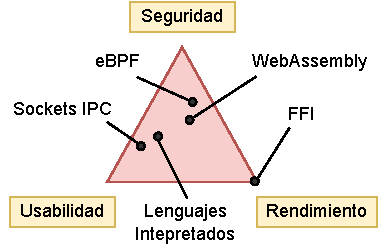
\includegraphics[width=10cm]{./Imagenes/triangle.pdf}
    \caption{Comparación aproximada de los métodos investigados.}%
    \label{fig:triangle}
\end{figure}
